% !TeX spellcheck = en_US
\chapter{Neural Network}
Deep neural network takes care of the complex feature engineering process (\charef{cha:feature-engineering}). \Eg, in classical computer vision, for people detection, the following process is applied:
\begin{enumerate}
	\item Input: Image
	\item Low-level feature extraction: \ac{HOG}
	\item Mid-level features: \ac{DPM}
	\item Classifier: \ac{SVM}
	\item Output: final label
\end{enumerate}
Using deep neural network, the process is truncated to simply:
\begin{enumerate}
	\item Input: Image
	\item Network training (end-to-end)
	\item Output: final label
\end{enumerate}
Different tasks require special expertise to design feature extraction, \eg, designing a program playing gammon would need someone knowing the rules, tips and tricks. On the other hands, we can assured that the human-proposed features are sufficient and helpful. Deep neural network alleviate the human-effort of hand-designing feature extraction process. In addition, it also learns prioritize important features for specific task.

\section{General}
\hlb{Forward pass:}
\begin{align}
	\textbf{y}^{(0)} &= \textbf{x}\\
	\textbf{z}^{(k)} &= \textbf{W}^{(k)}\textbf{y}^{(k-1)}, \qquad k = 1, \dots, l\\
	\textbf{y}^{(k)} &= g_k(\textbf{z}^{(k)})\\
	\textbf{y} &= \textbf{y}^{(l)}\\
	E &= L(\textbf{t}, \textbf{y}) + \lambda \Omega(\textbf{W})
\end{align}
\hlb{Backward pass:}
\begin{align}
	h \leftarrow &\frac{\partial E}{\partial \textbf{y}} = \frac{\partial}{\partial \textbf{y}} L(\textbf{t, y}) + \lambda \frac{\partial}{\partial \textbf{y}} \Omega\\
	\text{for } k =l \leftarrow &1:\\
	h \leftarrow &\frac{\partial E}{\partial \textbf{z}^{(k)}} = h \odot g(\textbf{y}^{(k)})\\
	&\frac{\partial E}{\partial \textbf{w}^{(k)}} = h \textbf{y}^{(k-1)T} + \lambda \frac{\partial \Omega}{\partial \textbf{w}^{(k)}}\\
	h \leftarrow &\frac{\partial E}{\partial \textbf{y}^{(k-1)}} = \textbf{W}^{(k)T} h
\end{align}

\section{Gradient Descent}
\note Just use ADAM??

\subsection{Vanilla Gradient Descent}
\begin{equation}
	\theta_{t+1} = \theta_t - \eta\nabla_\theta f(\theta_t)
\end{equation}
Check derivative:
\begin{equation}
	f'(x) \approx \frac{f(x+\varepsilon) - f(x-\varepsilon)}{2\varepsilon} \;\;\;\;\; \text{(numerical gradient)}
\end{equation}

\subsection{Momentum}
\begin{itemize}
	\item Init: $v_{dW_0} = 0, v_{db_0} = 0$
	\item Calculate $dW, db$
	\item Update $W, b$
	\begin{equation}
		\Rightarrow \begin{cases}
			v_{dW} &= \beta v_{dW} + (1-\beta)dW\\
			v_{db} &= \beta v_{db} + (1-\beta)db
		\end{cases}
		\Rightarrow
		\begin{cases}
			W &= W - \alpha v_{dW}\\
			b &= b - \alpha v_{db}
		\end{cases}
	\end{equation}
	The above formulas are to calculate the moving average of $v_{dW}$ and $v_{db}$.
	\item Tips: Choose \hlre{\beta_1=0.9}, implying taking average of the last 10 steps.
	\item Reference source: \href{https://youtu.be/k8fTYJPd3_I}{DeepLearning.AI}.
\end{itemize}

\subsection{Nesterov Accelerated Gradient}
\ac{nag}:
\begin{equation}
	v_t = \gamma v_{t-1} + \eta \nabla_tJ\left(\theta - \gamma v_{t-1}\right)
\end{equation}

\subsection{\ac{rmsprop}}
\begin{itemize}
	\item Init $s_{dW_0} = 0, s_{db_0}=0$
	\item Calculate $dW, db$
	\item Update $W, b$
	\begin{equation}
		\begin{cases}
			s_{dW} &= \beta s_{dW} + (1-\beta)dW^2 \\
			s_{db} &= \beta s_{db} + (1-\beta)db^2
		\end{cases}
		\Rightarrow
		\begin{cases}
			W &= W - \alpha \frac{dW}{\sqrt{s_{dW}} + \varepsilon}\\
			b &= b - \alpha \frac{db}{\sqrt{s_{db}} + \varepsilon}
		\end{cases}
	\end{equation}
	\item Tips: choose \hlre{\beta_2 = 0.999, \;\;\varepsilon = 10^{-7}}
	\item Reference source: \href{https://youtu.be/_e-LFe_igno}{DeepLearning.AI}.
\end{itemize}

\subsection{\ac{adam}}
\ac{adam} is basically the combination of Momentum and \ac{rmsprop}.
\begin{itemize}
	\item Init $v_{dW_0}, s_{dW_0}, v_{db_0}, s_{db_0}=0$
	\item Calculate $dW, db$
	\item Update $W, b$
	\begin{equation}
		\begin{cases}
			v_{dW} &= \beta_1 v_{dW} + (1-\beta_1)dW \\
			v_{db} &= \beta_1 v_{db} + (1-\beta_1)db \\
			s_{dW} &= \beta_2 s_{dW} + (1-\beta_2)dW^2 \\
			s_{db} &= \beta_2 s_{db} + (1-\beta_2)db^2
		\end{cases}
		\Rightarrow
		\begin{cases}
			v^{cor.}_{dW} &= \frac{v_{dW}}{1 - \beta_1^t} \\
			v^{cor.}_{db} &= \frac{v_{db}}{1 - \beta_1^t} \\
			s^{cor.}_{dW} &= \frac{s_{dW}}{1 - \beta_2^t} \\
			s^{cor.}_{db} &= \frac{s_{db}}{1 - \beta_2^t}
		\end{cases}
		\Rightarrow
		\begin{cases}
			W &= W - \alpha \frac{v^{cor.}_{dW}}{\sqrt{s^{cor.}_{dW}} + \varepsilon}\\
			b &= b - \alpha \frac{v^{cor.}_{db}}{\sqrt{s^{cor.}_{db}} + \varepsilon}
		\end{cases}
	\end{equation}
	\item Tips: choose \hlre{\beta_1 = 0.9, \quad\beta_2 = 0.999, \quad\varepsilon = 10^{-7}}
	\item Reference source: \href{https://youtu.be/JXQT_vxqwIs}{DeepLearning.AI}.
\end{itemize}

\section{Tips and Tricks}

\begin{itemize}
	\item Shuffling
	\item Data Augmentation: reshape, rescale, crops, zooming, change color (color \ac{PCA})
	\item Normalizing the inputs\\
	Convergence is the fastest if
	\begin{itemize}
		\item The mean of each input variable $=0$
		\item Scale $\Rightarrow$ same covariance
	\end{itemize}
	Mean cancellation $\Rightarrow$ \ac{KL} expansion $\Rightarrow$ covariance equalization (if possible)
	\item Leaky \ac{relu} is better a bit than \ac{relu}, ELU
	\item Weights initialization: Xavier-Glorot:
	\[ W \sim U\left(0, \sqrt{\frac{6}{n_{in} + n_{out}}}\right) \]
	\item Batch Norm(alization): Normalize after each layer\\
	$\Rightarrow$ learn the moving average
	\item Drop out\\
	\note When in inferencing (after training), must multiply the activation output with the \ac{prob} that the weights are set to 0
\end{itemize}

\section{Network Structures}
This section present some common network structures and their capabilities.

\subsection{Recurrent Neural Network}
\ac{BPTT}:\\
\todo{Add image, content}
\begin{align}
	\frac{\partial E_t}{\partial w_{ij}} &= \sum_{1 \leq k \leq t} \left( \frac{\partial E_t}{\partial h_t} \frac{\partial h_t}{\partial h_k} \frac{\partial h_k}{\partial w_{ij}} \right)\\
	E &= \sum_{1 \leq t \leq T} E_t\\
	\frac{\partial h_t}{\partial h_k} &= \prod_{t \geq i \geq k} \frac{\partial h_i}{\partial h_{i-1}}
\end{align}

\subsection{Residual Network}
\todo{Residual:}
\begin{figure}[hbt!]
	\centering
	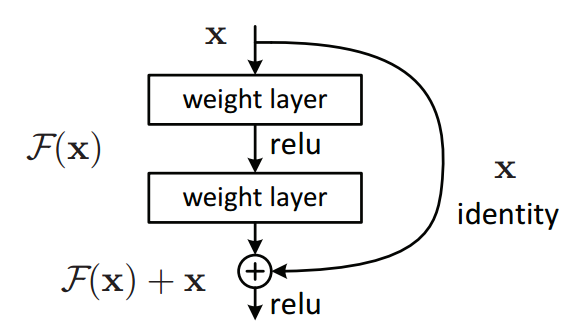
\includegraphics[width=0.5\textwidth]{residual-modul.png}
	\caption{Residual block (\href{https://www.google.com}{\todo{}}).}
\end{figure}